\documentclass[12pt]{beamer}
%\documentclass[20pt,handout]{beamer}
\usetheme{Darmstadt}
\usepackage{graphicx}
%\usepackage[german]{babel}
\usepackage{ngerman}
\usepackage[T1]{fontenc}
\usepackage[utf8]{inputenc}
\usepackage{tikz}
\setbeamertemplate{footline}[frame number]

\newcommand{\cc}[1]{\includegraphics[height=4mm]{img/#1.png}\hspace{1mm}}
\usepackage{ifthen}
\newcommand{\license}[2][]{\\#2\ifthenelse{\equal{#1}{}}{}{\\\scriptsize\url{#1}}}
\usepackage{textcomp}
\usepackage{hyperref}

\pgfdeclareimage[height=.6cm]{c3d2logo}{./img/c3d2.pdf}


\pgfdeclarelayer{foreground}
\pgfsetlayers{main,foreground}
\logo{\pgfputat{\pgfxy(-1,0)}{\pgfbox[center,base]{\pgfuseimage{c3d2logo}}}}


\title{Wie schütze ich mich vor Überwachung?}
\author{\small Marius Melzer und Paul Schwanse\\\large Chaos Computer Club Dresden}
\date{25.08.2015}

\begin{document}
\maketitle

\section{Einleitung}
\subsection{}

\begin{frame}
    \frametitle{Chaos Computer Club}
    \begin{center}
	\includegraphics[height=0.2\textheight]{img/chaosknoten.png}
    \end{center}	
    \begin{itemize}
      \item<1-> Verein wurde 1981 gegr"undet (\url{https://ccc.de})          
      \item<2-> Aktuell ca. 4500 Mitglieder
      \item<3-> Betreibt u.a. "Offentlichkeitsarbeit und Politikberatung      
    \end{itemize}
\end{frame}

\begin{frame}
  \frametitle{Chaos Computer Club}
  \begin{figure}
    \includegraphics[height=0.7\textheight]{img/fingerabdruck.jpg}
  \end{figure}
\end{frame}

\begin{frame}
  \frametitle{Chaos Computer Club}
  \begin{figure}
    \includegraphics[height=0.7\textheight]{img/trojaner.png}
  \end{figure}
\end{frame}

\begin{frame}
    \frametitle{Chaos Computer Club}
    \begin{center}
	\includegraphics[height=0.1\textheight]{img/c3d2_logo.png}
    \end{center}
    \begin{itemize}
      \item<1-> Chaos Computer Club Dresden (\url{https://c3d2.de})          
      \item<2-> Datenspuren: 24./25. Oktober 2015 (\url{https://datenspuren.de})
      \item<3-> Podcasts (\url{https://c3d2.de/radio.html})
      \item<4-> Chaos macht Schule (\url{https://c3d2.de/schule.html})
    \end{itemize}
\end{frame}

\begin{frame}
    \frametitle{Bundespräsident Gauck zur NSA-Überwachung}
    \begin{center}
      ``Wir wissen z.B., dass es nicht so ist, wie bei der Stasi und dem KGB, dass es dicke Aktenbände gibt, wo unsere Gesprächsinhalte alle aufgeschrieben und schön abgeheftet sind. Das ist es nicht.''
      (Gauck, 30.06.2013 im ZDF-Sommerinterview)
    \end{center}
\end{frame}

\begin{frame}
    \frametitle{NSA-Skandal}
    \begin{center}
	\includegraphics[height=0.7\textheight]{img/snowden.jpg}
	\\{\small \href{https://commons.wikimedia.org/wiki/File:Edward_Snowden.jpg\#mediaviewer/File:Edward_Snowden-2.jpg}{Grafik}: \href{https://creativecommons.org/licenses/by/3.0/}{\cc{by}} Laura Poitras / Praxis Films}
    \end{center}	
\end{frame}

\begin{frame}
    \frametitle{Stasi vs. NSA}
    \begin{center}
      \includegraphics[height=0.7\textheight]{img/akten1.png}
    \end{center}
\end{frame}

\begin{frame}
    \frametitle{Stasi vs. NSA}
    \begin{center}
      \includegraphics[height=0.7\textheight]{img/akten2.png}
    \end{center}
\end{frame}

\section{Internet}
\subsection{}

\begin{frame}
    \frametitle{Routing im Internet}
    \begin{center}
      \includegraphics[height=0.7\textheight]{img/internet_cable_map.png}
    \end{center}
\end{frame}

\begin{frame}
    \frametitle{Internet-Verbindungen}
    \begin{center}
      \includegraphics[height=0.7\textheight]{img/internetmap-abhoeren}
    \end{center}
\end{frame}

\section{Verschlüsselung}
\subsection{}

\begin{frame}
    \frametitle{Tempora}
    \includegraphics[height=0.7\textheight]{img/spiegel-tempora.png}
\end{frame}

\begin{frame}
    \frametitle{Datenverlust auf dem Weg}
    \begin{center}
      \includegraphics[height=0.7\textheight]{img/internetmap-abhoeren-tempora}
    \end{center}
\end{frame}

\begin{frame}
    \frametitle{Datenverlust auf dem Weg}
    \begin{center}
      \includegraphics[height=0.7\textheight]{img/internetmap-abhoeren-ssl}
    \end{center}
\end{frame}

\begin{frame}
    \frametitle{Verschlüsselung}
    \begin{center}
	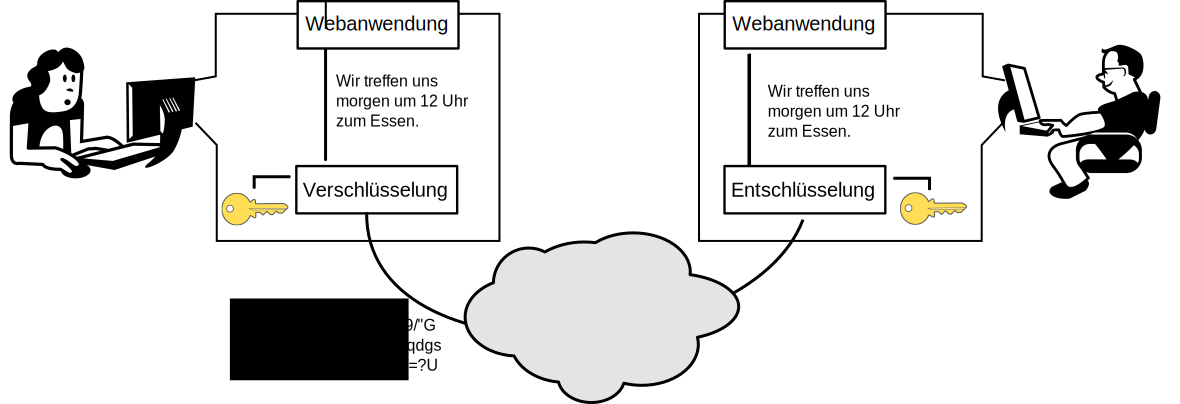
\includegraphics[width=\textwidth]{img/krypto.pdf}
    \end{center}	
\end{frame}

\begin{frame}
    \frametitle{Transportwegverschlüsselung}
      SSL = Secure Socket Layer / TLS = Transport Layer Security
    \vfill
    \begin{center}
      
\includegraphics[width=0.8\textwidth]{img/tls.pdf}
    \end{center}
\end{frame}

\begin{frame}
    \frametitle{SSL im Browser}
    \begin{center}
	\includegraphics[height=0.7\textheight]{img/ssl_verified.png}
    \end{center}
\end{frame}

\begin{frame}
    \frametitle{SSL im Browser}
    \begin{center}
	\includegraphics[height=0.7\textheight]{img/ssl_special.png}
    \end{center}
\end{frame}

\begin{frame}
    \frametitle{SSL im Browser}
    \begin{center}
	\includegraphics[height=0.7\textheight]{img/ssl_unverified.png}
    \end{center}
\end{frame}

\begin{frame}
  \frametitle{HTTPS Everywhere}
    \begin{center}
      \includegraphics[height=5cm]{img/https-everywhere.png}
    \end{center}
\end{frame}
%% http://www.theconnectivist.com/2013/06/the-expanding-consolidation-of-the-consumer-internet/

\begin{frame}
    \frametitle{Datenverlust beim Dienst}
    \begin{center}
      \includegraphics[height=0.7\textheight]{img/internetmap-abhoeren-prism-ssl}
    \end{center}
\end{frame}

\begin{frame}
    \frametitle{Prism}
    \begin{center}
      \includegraphics[height=0.7\textheight]{img/prism.jpg}
    \end{center}
\end{frame}

\begin{frame}
  \frametitle{Ende-zu-Ende-Verschlüsselung}
  \begin{itemize}
    \item<1-> GPG für E-Mails
    \item<2-> OTR für Jabber:
      \begin{itemize}
        \item Pidgin mit OTR-Plugin für Linux und Windows
        \item GibberBot oder Xabber für Android
        \item Adium für Mac, ChatSecure für iOS
      \end{itemize}
    \item<3-> palava.tv oder Linphone für Videotelefonie
    \item<4-> Redphone für Handytelefonate (Android)
    \item<5-> TextSecure für Nachrichten (Android)
  \end{itemize}
\end{frame}

\begin{frame}
  \frametitle{E-Mail-Selbstverteidigung}
  \begin{center}
    \includegraphics[height=0.5\textheight]{img/emailselfdefense.png}
    \begin{itemize}
      \item https://emailselfdefense.fsf.org/de/
    \end{itemize}	
  \end{center}	
\end{frame}

\begin{frame}
  \frametitle{TextSecure}
    \begin{center}
      \includegraphics[height=6cm]{img/textsecure1.png}
      \hspace{0.5cm}
      \includegraphics[height=6cm]{img/textsecure2.png}
    \end{center}
\end{frame}

\section{Metadaten}
\subsection{}

\begin{frame}
  \frametitle{Metadaten}
  \begin{itemize}
    \item Handynetz
      \begin{itemize}
        \item Telefonnummern
        \item Zeitpunkt und Dauer (Telefonate, SMS)
        \item Funkzelle (Ort)
      \end{itemize}
    \item Internet
      \begin{itemize}
        \item IP-Adresse (= ungefährer Ort)
        \item Alle Verbindungen
        \item Email: Adressen von Sender und Empfänger, Zugriff
      \end{itemize}
  \end{itemize}
\end{frame}

\begin{frame}
    \frametitle{Metadaten}
    \begin{center}
      \includegraphics[height=0.7\textheight]{img/wekillpeople.jpg}
    \end{center}
\end{frame}

\begin{frame}
  \frametitle{Tor (zum Verstecken des Orts)}
  \begin{center}
    \includegraphics[height=0.5\textheight]{img/tor-banner.png}
  \end{center}
\end{frame}

\begin{frame}
  \frametitle{Tor (zum Verstecken des Orts)}
  \begin{center}
    \includegraphics[height=0.5\textheight]{img/internetmap-abhoeren-tor}
  \end{center}
\end{frame}

\begin{frame}
  \frametitle{Tor Browser}
  \begin{center}
    \includegraphics[height=0.8\textheight]{img/torbrowser1.png}
  \end{center}
\end{frame}

\begin{frame}
  \frametitle{Tor Browser Plugins}
  \begin{center}
    \includegraphics[height=0.6\textheight]{img/torbrowser2.png}
  \end{center}
\end{frame}

\begin{frame}
    \frametitle{Metadaten - Aufgerufene Websites}
    \begin{center}
      \includegraphics[height=0.7\textheight]{img/lightbeam.png}
      \\{\small \href{http://www.flickr.com/photos/8517757@N03/10538205035/in/photolist-h4e4dg}{Grafik:} \href{http://creativecommons.org/licenses/by-sa/3.0/deed.en}{\cc{by-sa}} Clint Lalonde}
    \end{center}
\end{frame}

\begin{frame}
  \frametitle{Disconnect, Privacy Badger, Ghostery}
  \begin{center}
    \includegraphics[height=0.7\textheight]{img/disconnectme.jpg}
  \end{center}
\end{frame}

\section{Soziale Netzwerke}
\subsection{}

\begin{frame}
  \frametitle{Soziale Netzwerke}
  \begin{itemize}
    \item Wer nutzt was?
      \begin{itemize}
        \item<2-> Facebook
        \item<3-> Twitter
        \item<4-> Whatsapp
        \item<5-> Instagram
        \item<6-> Snapchat
        \item<7-> Andere?
      \end{itemize}
  \end{itemize}
\end{frame}

\begin{frame}
  \frametitle{Firmen}
  \begin{itemize}
    \item Womit verdienen folgende Firmen ihr Geld?
      \begin{itemize}
        \item<2-> Karstadt
        \item<3-> Amazon
        \item<4-> Ebay
        \item<5-> Facebook
      \end{itemize}
  \end{itemize}
\end{frame}

\begin{frame}
  \frametitle{Gesch"aftsmodelle}
  \begin{figure}
    \includegraphics[height=0.7\textheight]{img/business_pigs.jpg}
  \end{figure}
\end{frame}

\begin{frame}
  \frametitle{Soziale Netzwerke}

  \begin{itemize}
    \item Was haben soziale Netzwerke von euch?\\(am Bsp. von Facebook)
      \begin{itemize}
        \item<2-> 82\% Einnahmen aus Werbung
        \item<3-> 30\% Anteil an "`Facebook-Einkäufen"'
        \item<4-> durchschnittlich 1€/Profil
        \item<5-> "`Poweruser"'-Profile deutlich mehr
        \item<6-> => Mehr Werbegewinn durch personalisierte Werbung
        \item<7-> Q2 2014 791 Mio Dollar Gewinn
      \end{itemize}
  \end{itemize}
\end{frame}

\begin{frame}
    \frametitle{Soziale Netzwerke}
    \begin{itemize}
        \item<2-> Das Internet vergisst nichts!
        \item<3-> Was sollte man (nicht) schreiben?
        \item<5-> Wer soll meine Infos (nicht) erhalten?
        \item<6-> Beeinträchtigt was ich schreibe andere?
    \end{itemize}
\end{frame}

\begin{frame}
  \frametitle{Umgangsformen}
  \begin{itemize}
    \item Wem sollte man was preisgeben (und was eher nicht)?
      \begin{itemize}
        \item<2-> "`Roadkill"' von Entertainment for the Braindead ist ein cooles Album
        \item<3-> Ich gehe am Donnerstag, den 07.06.2012 ins Kino
        \item<4-> Ich bin heut' echt gut drauf!
        \item<5-> Ute Meyer war mit Carolin Wittich und Frederik Ulm am Samstag Abend in der Sportsbar und ist danach mit Michael Müller nach Hause gefahren
        \item<6-> Meine Lehrerin ist voll doof!
      \end{itemize}
  \end{itemize}
\end{frame}

\section{Verhalten}
\subsection{}

\begin{frame}
    \frametitle{Datensparsamkeit}
    \begin{itemize}
        \item<2-> Viele Daten zusammen ergeben Profile
        \item<3-> Verteilen der Daten, Nutzung mehrerer Dienste
        \item<4-> Werden die Daten gebraucht?
        \item<5-> Werden echte Daten gebraucht?
          \begin{itemize}
            \item<6-> Pseudonymität
            \item<7-> mailinator.com (Wegwerf-Email-Adresse)
            \item<8-> frank-geht-ran.de (Wegwerf-Telefonnummer)
            \item<9-> bugmenot.com (Fake Accounts)
          \end{itemize}
    \end{itemize}
\end{frame}

\begin{frame}
    \frametitle{Alternative Suchmaschinen}
    \begin{columns}
        \begin{column}{5cm}
            \begin{center}
                    \begin{itemize}
                            \item Startpage
                            \vspace{2cm}
                            \item DuckDuckGo
                    \end{itemize}
            \end{center}
        \end{column}
        \begin{column}{5cm}
            \begin{center}
                \includegraphics[width=0.5\textwidth]{img/startp_logo.png}
                \vspace{1cm}
                \includegraphics[width=0.8\textwidth]{img/duckduckgo.pdf}
            \end{center}
        \end{column}
    \end{columns}
\end{frame}

\begin{frame}
    \frametitle{Alternative Kartendienste}
    \begin{columns}
        \begin{column}{5cm}
            \begin{center}
                    \begin{itemize}
                            \item OpenStreetMap
                            \vspace{2cm}
                            \item OpenRouteService
                    \end{itemize}
            \end{center}
        \end{column}
        \begin{column}{5cm}
            \begin{center}
                \includegraphics[width=0.5\textwidth]{img/osm.png}
                \vspace{1cm}
                \includegraphics[width=0.8\textwidth]{img/openrouteservice.png}
            \end{center}
        \end{column}
    \end{columns}
\end{frame}

\begin{frame}
    \frametitle{Passwörter}
    \begin{itemize}
        \item<2-> Keine einfachen Wörter
        \item<3-> Groß-, Kleinbuchstaben, Ziffern, Sonderzeichen
        \item<4-> Beispiele:
            \begin{itemize}
                \item<5-> dragon
                \item<6-> (nCuAj.§Tsm!f
                \item<7-> IchLiebeDich
                \item<8-> .§)=/)=`
                \item<9-> qwerty
                \item<10-> Mks?o/.u,1Psw!
            \end{itemize}
        \item<12-> Verschiedene Passwörter nutzen!
        \item<13-> Passwort-Manager verwenden \\ (z.B. Keepass, Password Safe)
    \end{itemize}
\end{frame}

\begin{frame}
    \frametitle{Zusammenfassung}
    \begin{itemize}
        \item<2-> Verschlüsselung nutzen (SSL für Weg, Ende-zu-Ende für untereinander)
        \item<3-> Metadaten vermeiden (Tor, Disconnect Plugin)
        \item<4-> Sichere Passwörter nutzen
        \item<5-> Datensparsamkeit (was poste ich, Wegwerfemailadressen, etc.)
        \item<6-> Verletze nicht die Privatsphäre anderer (Frage nach!)
        \item<7-> Das Internet vergisst nichts
    \end{itemize}
\end{frame}

\begin{frame}
  \frametitle{Diskussion}
  \begin{center}
    {\Large Diskussion}\\
    \vspace{5mm}
    \href{https://github.com/c3d2/cms-nsa}{Folien}: \href{https://creativecommons.org/licenses/by-sa/4.0/}{\cc{by-sa}} Chaos Computer Club Dresden \\
    \vspace{4mm}
    CMS Dresden: schule@c3d2.de
  \end{center}
\end{frame}

\end{document}
